% ============================================================
%  TASK 5 — PCB LAYOUT AND FINAL CONCLUSION
% ============================================================

\section{Task 5: PCB Layout in KiCad}
\label{sec:kicad_layout}

To bridge the gap between simulations and a real-world energy harvesting system, the final step of this project involved designing the physical Printed Circuit Boards. 

Although the two-diode voltage doubler was identified as the optimal topology for reaching the \SI{1.5}{\volt} threshold, we decided to lay out and manufacture \textbf{both the 1-diode and 2-diode pure microstrip rectifiers}. Having both physical boards will allow for a direct comparison of their actual efficiencies.

\subsection{Design Constraints and Component Selection}

The routing was performed using the KiCad EDA software. To maintain strict fidelity with our ADS simulations, the PCBs were designed for a \textbf{Rogers 4350B substrate} ($H = \SI{1.6}{\milli\meter}$, $\epsilon_r = 4.5$). The bottom layer is a solid copper layer acting as the continuous ground plane required for microstrip transmission lines, while the top layer hosts the RF traces and components.

During the footprint assignment phase, we encountered a practical limitation: the specific footprint for the STTS22H temperature sensor was unavailable in standard libraries. We searched for solutions to implement it in Kicad but we finally replaced it by a \textbf{TPS3839} ultra-low power voltage supervisor in a standard \textbf{SOT-23} package. This component has more or less similar ultra-low current consumption characteristics and will act as an excellent representative dummy load to validate the DC power delivery of our rectennas.

\subsection{PCB 1: Single-Diode Microstrip Rectifier}

Figure~\ref{fig:PCB_1d} shows the 3D rendering of the single-diode board.

\begin{figure}[H]
    \centering
    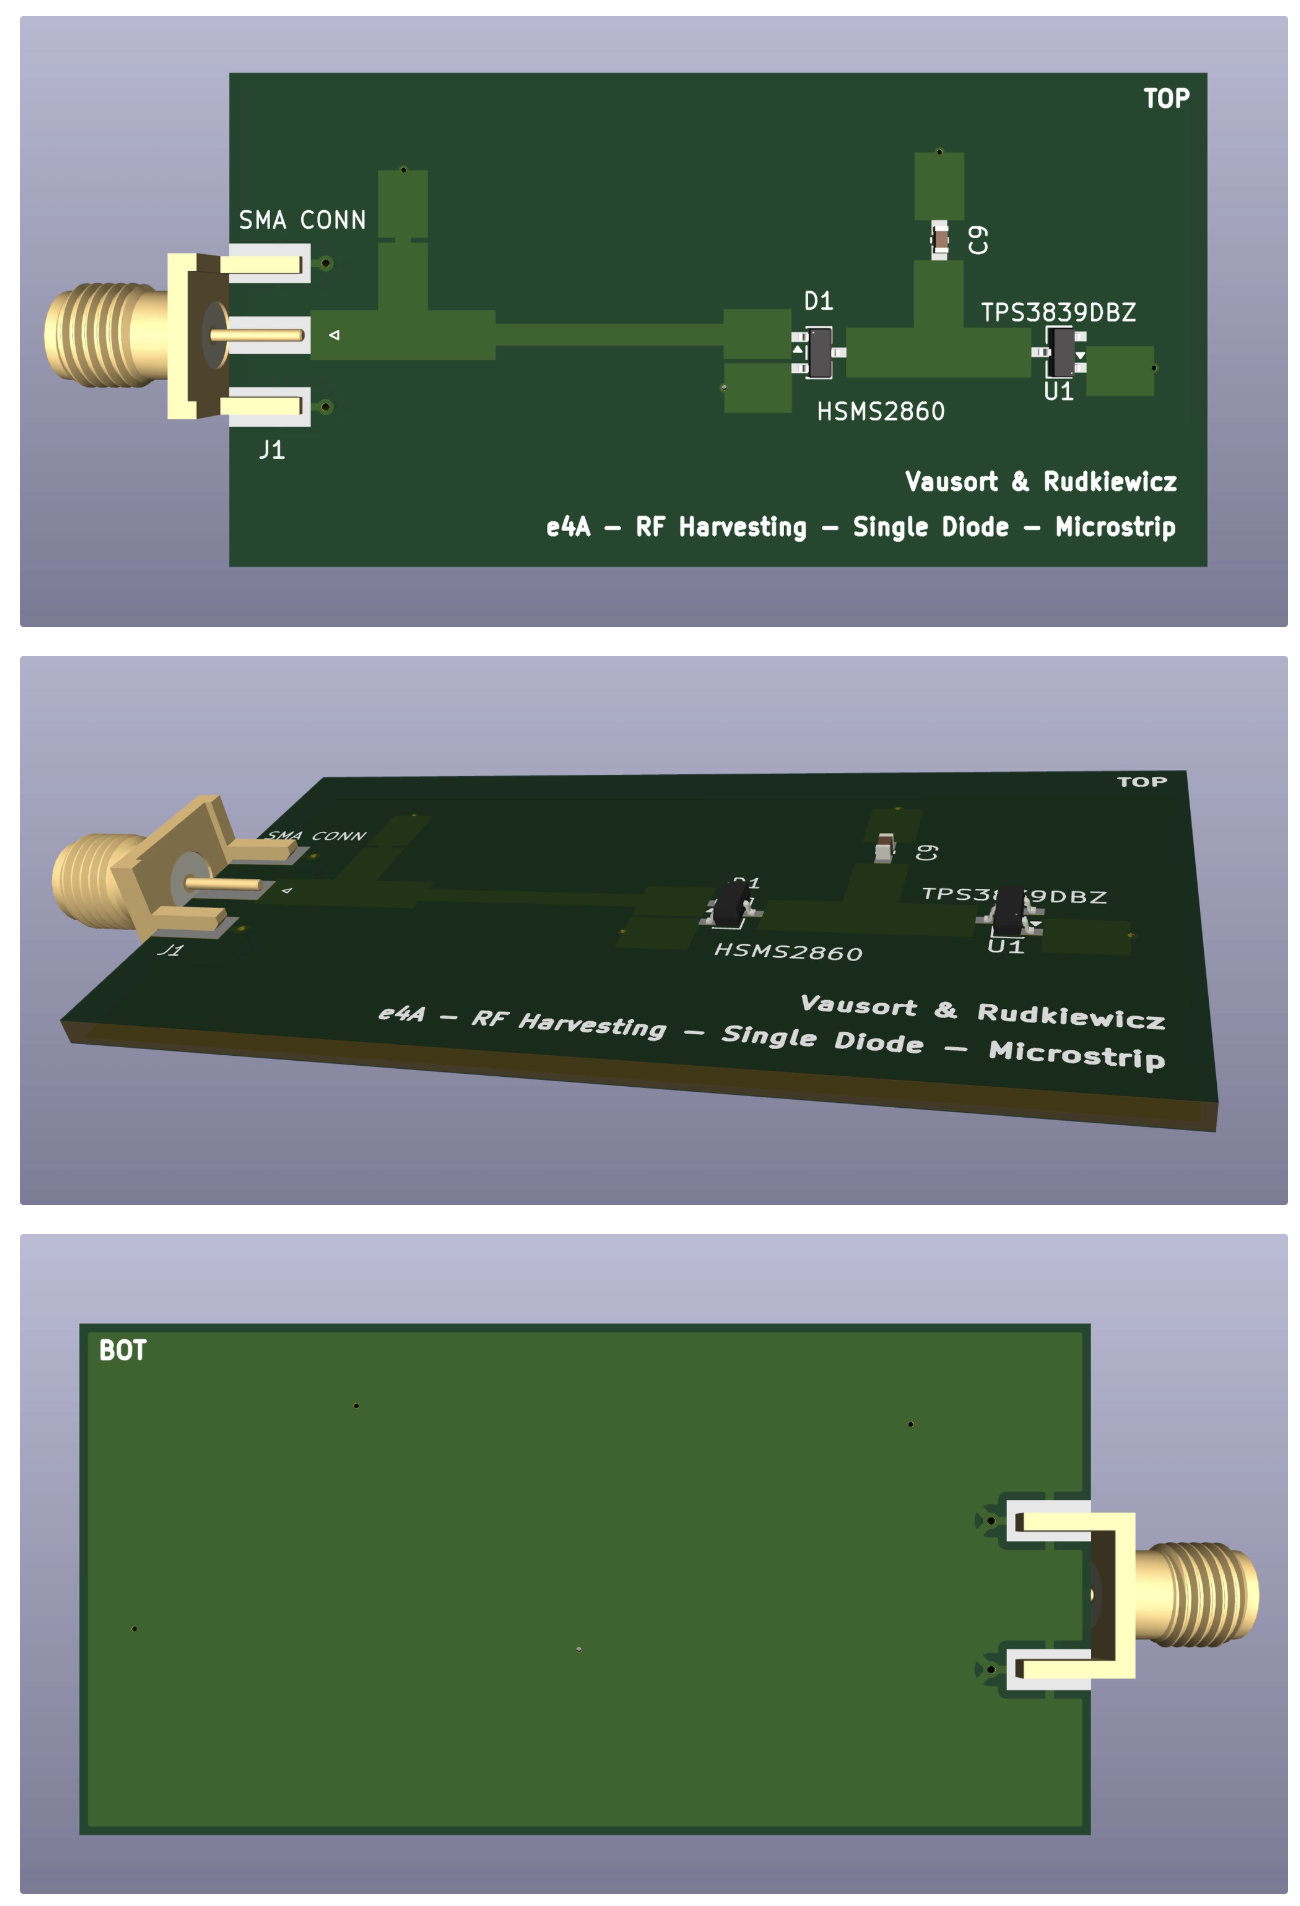
\includegraphics[width=\linewidth]{images/PCB_1d.png} 
    \caption{3D KiCad rendering of the Single-Diode Microstrip Rectifier (Top and Bottom views).}
    \label{fig:PCB_1d}
\end{figure}

The layout clearly shows the SMA input connector (J1) transitioning into the \SI{50}{\ohm} microstrip line, followed by the tuning lines. The signal is then rectified by the single \textbf{HSMS-2860} diode (D1) and filtered by the capacitor (C9) before reaching the TPS3839 dummy load (U1).

\subsection{PCB 2: Two-Diode Voltage Doubler Rectifier}

Figure~\ref{fig:PCB_2d} shows the 3D rendering of the two-diode voltage doubler board.

\begin{figure}[H]
    \centering
    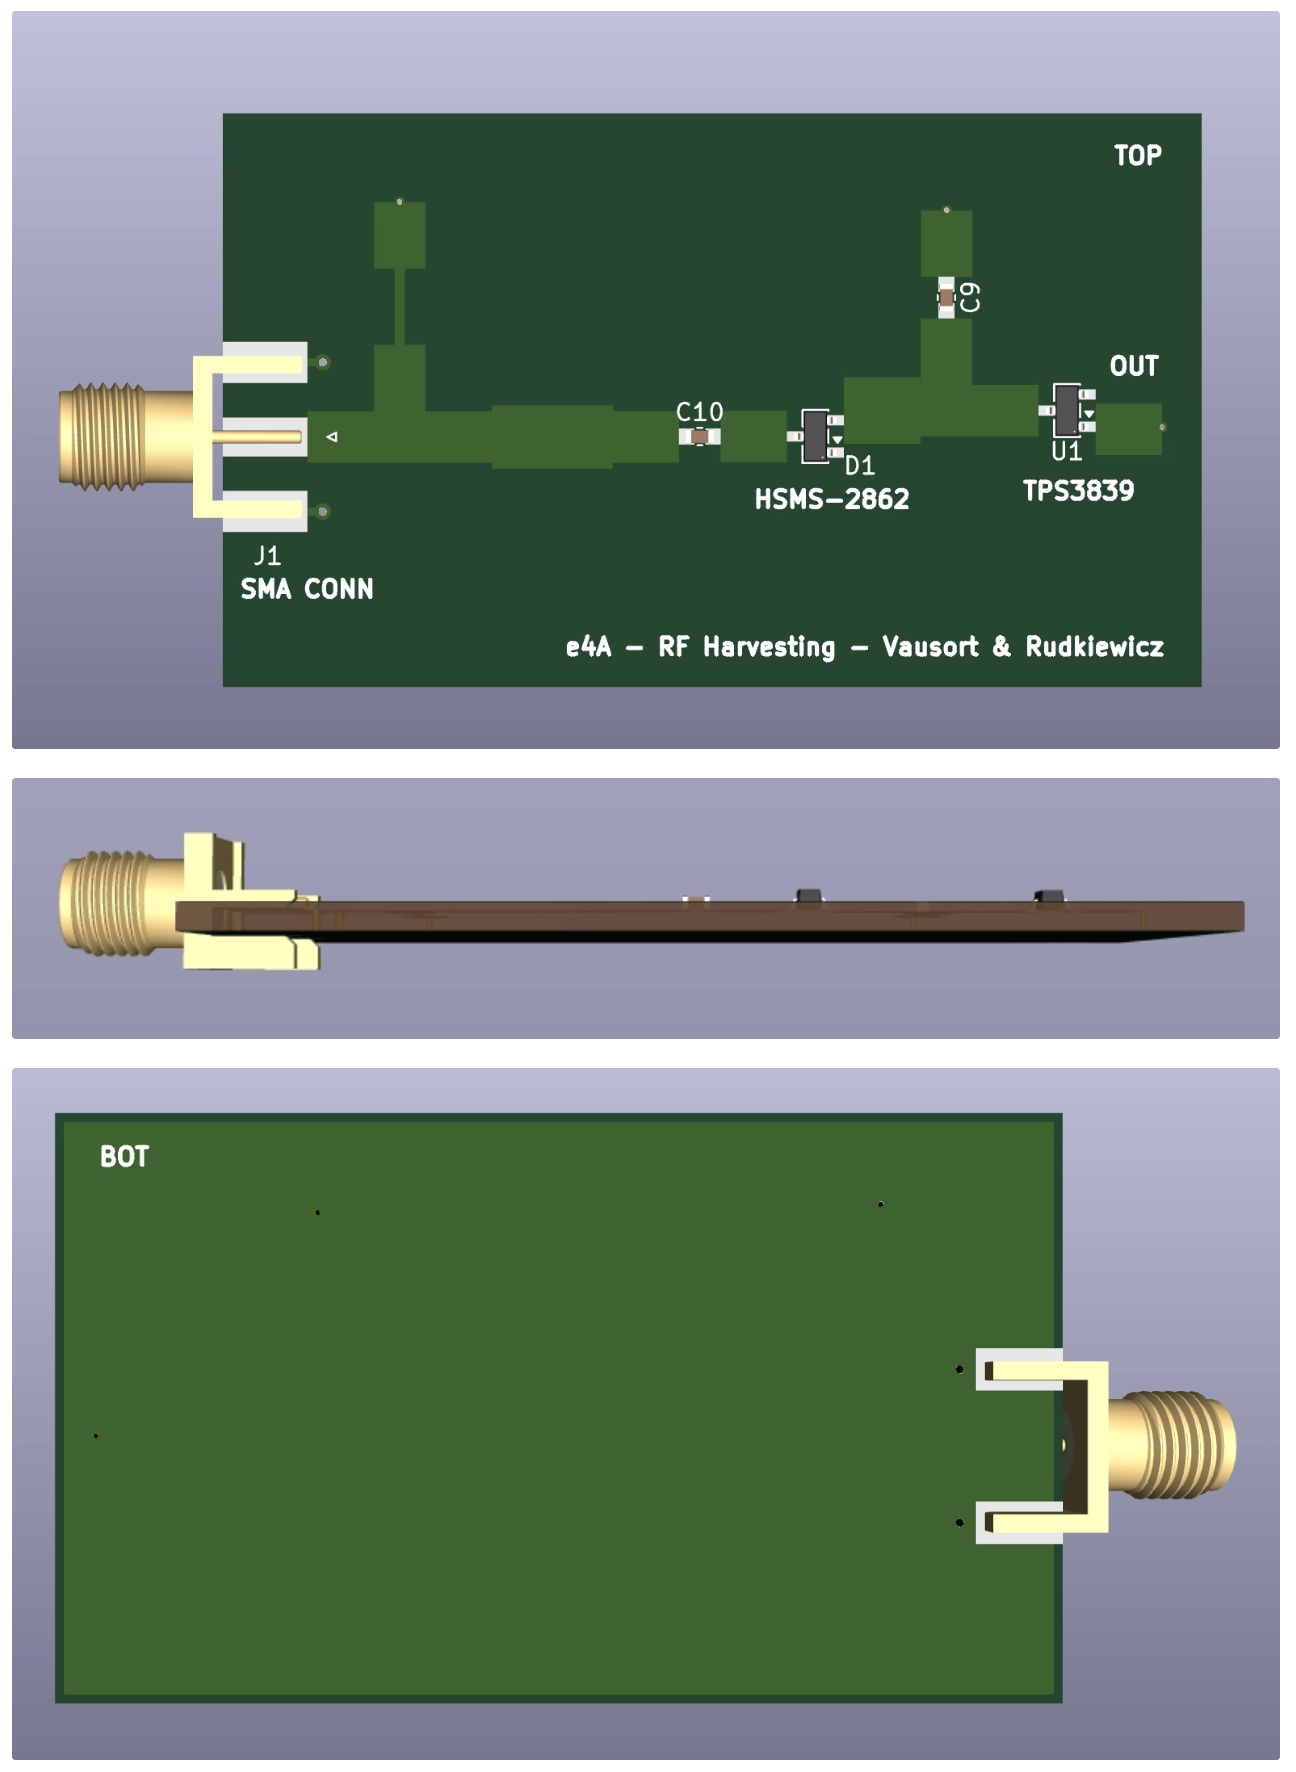
\includegraphics[width=\linewidth]{images/PCB_2d.png} 
    \caption{3D KiCad rendering of the Two-Diode Microstrip Voltage Doubler (Top and Bottom views).}
    \label{fig:PCB_2d}
\end{figure}

This board implements the more complex voltage doubler architecture. A series input capacitor (C10) separates the matching network from the rectification stage. We utilized the \textbf{HSMS-2862} component, minimiizing trace lengths and parasitic inductances between the two diodes. 

% ============================================================
%  FINAL CONCLUSION
% ============================================================

\section{Final Project Conclusion}
\label{sec:final_conclusion}

This project presented a comprehensive top-down engineering approach to designing an RF energy harvesting system operating at \SI{2.2}{\giga\hertz}. 

We successfully navigated through the entire RF design workflow:
\begin{enumerate}
    \item \textbf{Theoretical Modeling:} We extracted the non-linear, power-dependent complex impedance of Schottky diodes (HSMS-2860 and HSMS-2862) using Large-Signal S-Parameter (LSSP) simulations.
    \item \textbf{Impedance Matching:} We synthesized several matching networks, transitioning from ideal lumped LC components to physical, fully distributed microstrip topologies. We demonstrated how critical microstrip parameters (width, length, substrate thickness) affect the characteristic impedance.
    \item \textbf{Performance Evaluation:} Using Harmonic Balance (HB) simulations, we proved that while ideal LC circuits offer very high theoretical efficiencies (up to \textbf{66.5\%}), fully distributed microstrip circuits offer a much more reliable, component-free manufacturing path, despite a lower raw efficiency (\textbf{28.1\%}).
    \item \textbf{Application Targeting:} We showed the fundamental trade-off in energy harvesting, pure efficiency against usable voltage. We concluded that the two-diode voltage doubler, generates \SI{2.0}{\volt} at \SI{10}{\dBm}, is the only topology capable of reliably waking up our target ultra-low-power IoT load.
    \item \textbf{PCB Realization:} Finally, the optimized schematics were successfully routed into manufacturing-ready KiCad PCB layouts.
\end{enumerate}

The next logical step for this project will be to manufacture these boards, perform careful component soldering, and conduct physical measurements. Comparing the physical DC voltage measurements against our ADS simulation models will provide the validation of our RF energy harvesting design.